\documentclass[addpoints,12pt]{exam}
\usepackage[utf8]{inputenc}
\usepackage[spanish,es-noshorthands]{babel}
\usepackage{amsmath,amssymb}
\usepackage{graphicx}
\usepackage{array}
\usepackage{xcolor}
\usepackage{tikz}
\usetikzlibrary{calc,arrows.meta}
\usepackage[american]{circuitikz}
\usepackage[most]{tcolorbox}
\usepackage[legalpaper,margin=2cm,top=1.8cm]{geometry}

\graphicspath{{./}}
\definecolor{ubbblue}{RGB}{0,51,102}

\qformat{}
\newcommand{\qpts}[1]{{\setlength{\fboxsep}{2.5pt}\fbox{#1}}\hspace{0.6em}\ignorespaces}
\newcommand{\qhead}[1]{\thequestion.\hspace{0.5em}\qpts{#1}}
\newcommand{\pts}[1]{\textcolor{red}{\textbf{(#1 pts)}}}
\newcommand{\uF}{\ [\mu\mathrm{F}]}
\newcommand{\uC}{\ [\mu\mathrm{C}]}

% Lazo rectangular en el plano xy: #1 lado 12, #2 lado 23, #3 punta de flecha (-> antihorario, <- horario)
\newcommand{\figlazo}[3]{%
\begin{tikzpicture}[>=Stealth, line width=0.9pt,
    x={(1cm,0cm)}, y={(0.62cm,0.46cm)}, z={(0cm,1cm)}]
    \draw[->] (0,0,0) -- (#1+1.2,0,0) node[right]{$x$};
    \draw[->] (0,0,0) -- (0,#2+1.3,0) node[above right]{$y$};
    \draw[->] (0,0,0) -- (0,0,2.6) node[above]{$z$};
    \draw[line width=1.6pt] (0,0,0) -- (#1,0,0) -- (#1,#2,0) -- (0,#2,0) -- cycle;
    \fill (0,0,0) circle (1.6pt); \fill (#1,0,0) circle (1.6pt);
    \fill (#1,#2,0) circle (1.6pt); \fill (0,#2,0) circle (1.6pt);
    \node[below left]  at (0,0,0)    {$1$};
    \node[below right] at (#1,0,0)   {$2$};
    \node[right]       at (#1,#2,0)  {$3$};
    \node[above left]  at (0,#2,0)   {$4$};
    \draw[#3,red,line width=1.3pt] (0.35*#1,0,0) -- (0.65*#1,0,0);
    \draw[#3,red,line width=1.3pt] (#1,0.35*#2,0) -- (#1,0.65*#2,0);
    \draw[#3,red,line width=1.3pt] (0.65*#1,#2,0) -- (0.35*#1,#2,0);
    \draw[#3,red,line width=1.3pt] (0,0.65*#2,0) -- (0,0.35*#2,0);
    \node[red] at (0.5*#1,0.5*#2,0) {$I$};
    \node[below] at (0.5*#1,-0.1,0) {$a$};
    \node[right] at (#1+0.12,0.5*#2,0) {$b$};
\end{tikzpicture}}

\pagestyle{headandfoot}
\runningheadrule
\firstpageheader{}{}{}
\runningheader{\small F\'isica II - Electromagnetismo}%
              {\small\textbf{Certamen 3}}%
              {\small 30 de Octubre, 2026}
\firstpagefooter{}{\thepage}{}
\runningfooter{}{Page \thepage\ of \numpages}{}

\begin{document}

%========================================================
% PORTADA
%========================================================
\begin{center}
    
\includegraphics[height=1.9cm]{logo ubb.png}\hspace{1cm}%
    
\includegraphics[height=1.5cm]{logo dfis.png}\\[0.5cm]
    {\Large F\'isica II - Electromagnetismo}\\[0.15cm]
    {\LARGE\textbf{Certamen 3}}\\[0.9cm]
    30 de Octubre, 2026
\end{center}

\vspace{0.7cm}

\noindent\textbf{Nombre Completo}: \hrulefill\\[0.7cm]
\noindent\textbf{Rut}: \makebox[6.5cm]{\hrulefill}\hspace{0.3cm}\textbf{Carrera}: \hrulefill

\vspace{0.4cm}
\noindent\rule{\textwidth}{1pt}
\vspace{0.2cm}

\noindent\textbf{Algunas consideraciones para esta evaluaci\'on:}
\begin{itemize}\setlength\itemsep{2pt}
    \item El certamen 3 contiene \numpages\ p\'aginas (incluida la portada) y \numquestions\ preguntas,
          con un total de \numpoints\ puntos.
    \item Cada pregunta debe ser respondida por s\'olo una respuesta. En caso de presentar m\'as de
          una, se anulan las respuestas.
    \item \textbf{No est\'a permitido el uso de celulares o tablet en el desarrollo de esta
          evaluaci\'on. De ser sorprendido utilizando estos art\'iculos su evaluaci\'on ser\'a
          calificada con nota 1.0.}
    \item Buena suerte!
\end{itemize}

\noindent Seleccione con una \textbf{X} el nombre del profesor de su secci\'on:

\vspace{0.15cm}
\noindent
\begin{minipage}{0.49\textwidth}
\begin{tabular}{|l|p{1.1cm}|}
\hline
Prof.\ Diego Ram\'irez & \\ \hline
Prof.\ Mor\'in \'Ordenes & \\ \hline
Prof.\ Luis Liempi & \\ \hline
Prof.\ Luis Soto & \\ \hline
\end{tabular}
\end{minipage}%
\begin{minipage}{0.49\textwidth}
\begin{tabular}{|l|p{1.1cm}|}
\hline
Prof.\ Ismael C\'aceres & \\ \hline
Prof.\ Evelyn Riveros & \\ \hline
Prof.\ Arturo Fern\'andez & \\ \hline
~ & \\ \hline
\end{tabular}
\end{minipage}

\vspace{0.9cm}
\begin{center}
{\large\textbf{Puntaje}}\\[0.2cm]
\gradetable[v][questions]
\end{center}

\newpage

%========================================================
% PREGUNTAS
%========================================================
\begin{questions}

%--------------------------------------------------------
% PREGUNTA 1  (capacitores - version 1)
%--------------------------------------------------------
\question[20]
\begin{minipage}[t]{0.56\textwidth}
\vspace{0pt}
\qhead{20}La figura muestra un circuito con cinco capacitores de capacitancias
$C_1=6{,}0\uF$, $C_2=2{,}0\uF$, $C_3=3{,}0\uF$, $C_4=6{,}0\uF$ y $C_5=2{,}0\uF$, conectados a una
fuente de voltaje $V$ desconocido. Con un volt\'imetro se mide que el voltaje en $C_5$ es de
$3{,}0$ [V].
\end{minipage}\hfill
\begin{minipage}[t]{0.40\textwidth}
\vspace{0pt}
\centering
\begin{circuitikz}[scale=0.8]
    \draw (0,0) to[battery,invert, l=$V$] (0,4) to[C, l=$C_1$] (3,4);
    \draw (3,4) to[C, l=$C_2$] (3,0) to[short] (0,0);
    \draw (3,4) to[C, l=$C_3$] (6,4) to[C, l=$C_4$] (6,2) to[C, l=$C_5$] (6,0) to[short] (3,0);
\end{circuitikz}\\[2pt]
{\footnotesize Fig.\ 1.}
\end{minipage}

\medskip
\noindent\textbf{(a)} Reduzca el circuito paso a paso. En cada etapa, dibuje el circuito equivalente
y calcule su capacitancia hasta obtener la capacitancia equivalente final. \pts{10}

\vspace{11cm}
\noindent\textbf{(b)} Determine la carga de cada uno de los cinco capacitores. \pts{10}

\newpage

%--------------------------------------------------------
% PREGUNTA 2  (circuito resistivo - version 1)
%--------------------------------------------------------
\question[20]
\qhead{20}Considere el circuito compuesto de cinco resistencias y dos fuentes de voltaje que muestra
la figura, donde
\[
    R_1=R_3=2\ [\Omega],\quad R_2=4\ [\Omega],\quad R_4=R_5=8\ [\Omega],
    \qquad V_1=16\ [\mathrm{V}],\quad V_2=4\ [\mathrm{V}].
\]
\begin{center}
\begin{circuitikz}[american,scale=.88,transform shape]
\draw (0,0) to[battery1,invert,l_=$V_1$] (0,3)
 to[R,l=$R_1$,i>^=$I_1$] (3,3) node[circ]{}
 to[R,l=$R_3$,i>^=$I_3$] (6,3) node[circ]{}
 -- (8,3) to[R,l=$R_5$] (8,0) -- (6,0) node[circ]{};
\draw (3,3) to[R,l=$R_2$,i>^=$I_2$] (3,0) node[circ]{} -- (0,0);
\draw (6,3) to[R,l=$R_4$] (6,0);
\draw (3,0) to[battery1,l=$V_2$] (6,0);
\node at (-.35,2.1) {$+$}; \node at (-.35,.9) {$-$};
\node at (3.95,-.4) {$+$};  \node at (5.05,-.4) {$-$};
\end{circuitikz}\\[2pt]
{\footnotesize Fig.\ 2.}
\end{center}

\noindent\textbf{(a)} Determine la resistencia equivalente $R_{\mathrm{eq}}$ que se obtiene al reducir
las resistencias $R_3$, $R_4$ y $R_5$. Indique las combinaciones en serie y en paralelo utilizadas.
\pts{5}

\vspace{5cm}
\noindent\textbf{(b)} Aplicando las leyes de Kirchhoff, determine las corrientes $I_1$, $I_2$ e
$I_3$, con los sentidos indicados en la figura. \pts{6}

\vspace{7.5cm}
\noindent\textbf{(c)} Determine la corriente, la diferencia de potencial y la potencia disipada en
$R_1$, $R_2$ y $R_{\mathrm{eq}}$. Complete la tabla. \pts{9}

\begin{center}
\renewcommand{\arraystretch}{1.6}
\begin{tabular}{|c|>{\centering\arraybackslash}p{3cm}|>{\centering\arraybackslash}p{3cm}|>{\centering\arraybackslash}p{3cm}|}
\hline
Elemento & $I$ [A] & $\Delta V$ [V] & $P$ [W]\\ \hline
$R_1$ & & & \\ \hline
$R_2$ & & & \\ \hline
$R_{\mathrm{eq}}$ & & & \\ \hline
\end{tabular}
\end{center}

\newpage

%--------------------------------------------------------
% PREGUNTA 3  (fuerza magnetica - forma A)
%--------------------------------------------------------
\question[19]
\qhead{19}\textbf{(a)} Considere una carga puntual $q = -5\ [\mu\text{C}]$ que se mueve con rapidez
$v = 4\times10^{5}\ [\text{m/s}]$ en una regi\'on del espacio donde hay un campo magn\'etico de
intensidad $B = 0{,}02\ [\text{T}]$. Si las direcciones de la velocidad de la carga y del campo
magn\'etico se indican en la Fig.~3a, determine la fuerza magn\'etica $\vec{F}_m$ ejercida sobre la
carga puntual. \pts{7}

\begin{center}
    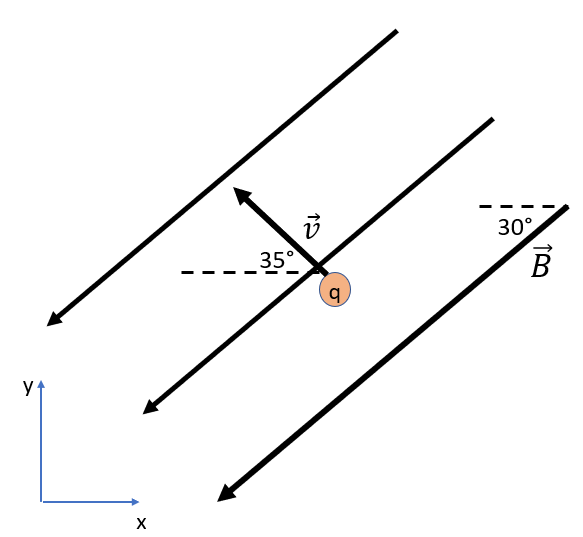
\includegraphics[width=0.42\textwidth]{fig3a.png}\\[2pt]
    {\footnotesize Fig.\ 3a.}
\end{center}

\newpage
\noindent\textbf{(b)} Considere un lazo de corriente de forma rectangular, de lados
$a = 8\ [\text{cm}]$ y $b = 5\ [\text{cm}]$, que se encuentra sobre el plano $xy$, como muestra la
Fig.~3b. Por el lazo circula una corriente $I = 2{,}5\ [\text{A}]$ en sentido antihorario y en la
regi\'on hay un campo magn\'etico $\vec{B} = 0{,}8\,\hat{\jmath} - 0{,}3\,\hat{k}\ [\text{T}]$.
Determine:

\begin{center}
    \figlazo{4.8}{3.0}{->}\\[2pt]
    {\footnotesize Fig.\ 3b.}
\end{center}

\noindent\textbf{(i)} La fuerza magn\'etica $\vec{F}_m$ sobre los tramos $12$ y $23$ del lazo de
corriente. \pts{6}

\vspace{8cm}
\noindent\textbf{(ii)} El momento magn\'etico $\vec{\mu}$ del lazo de corriente. \pts{3}

\vspace{4cm}
\noindent\textbf{(iii)} El torque magn\'etico $\vec{\tau}$ que ejerce el campo sobre la espira. \pts{3}

\end{questions}

\newpage

%========================================================
% FORMULARIO
%========================================================
\newtcolorbox{formbox}[1]{colback=gray!3, colframe=gray!55, coltitle=black,
    colbacktitle=white, fonttitle=\bfseries, boxrule=0.5pt, arc=2pt,
    left=6pt,right=6pt,top=2pt,bottom=2pt, before skip=4pt, after skip=4pt,
    title={#1}}
\setlength{\jot}{2pt}

\begin{center}{\large\textbf{Formulario}}\end{center}
\vspace{-0.1cm}

\begin{formbox}{Capacitancia}
\[
    C=\frac{Q}{\Delta V}
\]
\end{formbox}

\begin{formbox}{Capacitancia equivalente, cargas y voltajes}
\noindent
\begin{minipage}[t]{0.48\textwidth}
\centering\textbf{Serie}
\[
    \frac{1}{C_{eq}}=\frac{1}{C_1}+\frac{1}{C_2}+\cdots
\]
\[
    Q_1=Q_2=\cdots=Q
\]
\[
    \Delta V=\Delta V_1+\Delta V_2+\cdots
\]
\end{minipage}%
\hfill
\begin{minipage}[t]{0.48\textwidth}
\centering\textbf{Paralelo}
\[
    C_{eq}=C_1+C_2+\cdots
\]
\[
    \Delta V_1=\Delta V_2=\cdots=\Delta V
\]
\[
    Q=Q_1+Q_2+\cdots
\]
\end{minipage}
\end{formbox}

\begin{formbox}{Ley de Ohm y potencia disipada}
\[
    \Delta V=I\,R\ ;\qquad P=I\,\Delta V=I^2R=\frac{(\Delta V)^2}{R}
\]
\end{formbox}

\begin{formbox}{Resistencia equivalente}
\noindent
\begin{minipage}[t]{0.48\textwidth}
\centering\textbf{Serie}
\[
    R_{eq}=R_1+R_2+\cdots
\]
\end{minipage}%
\hfill
\begin{minipage}[t]{0.48\textwidth}
\centering\textbf{Paralelo}
\[
    \frac{1}{R_{eq}}=\frac{1}{R_1}+\frac{1}{R_2}+\cdots
\]
\end{minipage}
\end{formbox}

\begin{formbox}{Leyes de Kirchhoff}
\[
    \text{Nodos:}\ \ \sum I_{\text{entran}}=\sum I_{\text{salen}}
    \qquad\qquad
    \text{Mallas:}\ \ \sum_{\text{malla}}\Delta V=0
\]
\end{formbox}

\begin{formbox}{Fuerza magn\'etica sobre cargas y corrientes}
\[
    \vec{F}=q\,\vec{v}\times\vec{B}\ ;\qquad \vec{F}=I\,\vec{L}\times\vec{B}
\]
\end{formbox}

\begin{formbox}{Momento magn\'etico y torque magn\'etico}
\[
    \vec{\mu}=I\,A\,\hat{n}\ ;\qquad \vec{\tau}=\vec{\mu}\times\vec{B}
\]
\end{formbox}

\begin{formbox}{Prefijos}
$c=10^{-2}$, \quad $m=10^{-3}$, \quad $\mu=10^{-6}$, \quad $n=10^{-9}$, \quad $p=10^{-12}$.
\end{formbox}

\end{document}
